% -*- TeX-engine: luatex -*-
\documentclass[dvipsnames,presentation,aspectratio=169,14pt]{beamer}
\usepackage{hastingstheme}
\usepackage{qrcode}
\titlegraphic{
\includegraphics[scale=.35]{static_figures/du_bn.pdf}}
\author{\large Massimiliano Fasi}
\date{}

% \usepackage{template}
% \renewcommand{\authorname}{Lawrence Mitchell\inst{*}}
\renewcommand{\authoremail}{\inst{*}\texttt{lawrence.mitchell@durham.ac.uk}}

% \renewcommand{\sessionnumber}{2}
% \renewcommand{\sessiontitle}{Memory hierarchy}


\usetikzlibrary{matrix,fit,positioning,calc}
\usepackage{pgfplots}
% \pgfplotsset{compat=1.15}
\usepackage{pgfplotstable}
% \date{}


\begin{document}

\title{\firasemibold\color{White}%
  {\fontsize{20}{0}\selectfont SESSION 2\\
    \fontsize{40}{40}\selectfont Memory\\hierarchy\par}}
\titleslide

\begin{frame}
  \frametitle{Sum reduction benchmark (Exercise 1)}

  \begin{columns}[c]
    \begin{column}{0.27\textwidth}
      \small
      \vskip -50pt
      \begin{itemize}[itemsep=5pt,wide=0pt]
      \item SIMD: 4 plateaus
      \item scalar: 3 plateaus
      \end{itemize}
    \end{column}
    \begin{column}{0.7\textwidth}
      \begin{center}
        \vskip -10pt
        \begin{tikzpicture}
          \begin{axis}[
            height=7cm,
            width=10cm,
            xlabel={Bytes},
            ylabel near ticks,
            ylabel={MFlops/s},
            xmode=log,
            xtick={1e3,16e3,256e3,4e6,64e6},
            xticklabels={1kB,16kB,256kB,4MB,64MB},
            log basis x={10},
            style={font=\small},
            legend pos={north east},
            thick,
            legend style={
              cells={anchor=west, align=left},
              fill=bgcolor, font=\footnotesize}
            ]
            \pgfplotstableread[row sep=\\]{%
              Bytes scalar avx\\
              1 4646.58 25445.45\\
              2 4493.15 35128.01\\
              4 4450.96 40301.73\\
              8 4396.00 37515.23\\
              16 4360.66 36124.93\\
              32 4248.95 34167.31\\
              64 4075.51 25472.69\\
              128 4105.88 25863.90\\
              256 4107.04 26025.63\\
              512 3510.62 13717.75\\
              1024 2538.08 4760.64\\
              2048 2425.87 4540.75\\
              4096 2384.14 4595.67\\
              8192 764.49 3051.13\\
              16384 785.51 1041.38\\
              32768 763.71 1054.96\\
              65536 770.85 1020.18\\
              131072 770.84 1016.59\\
            }\mydata

            \addplot+ table[x=Bytes,y=scalar, thick] {\mydata};
            \addlegendentry{\texttt{sp\_sum}}

            \addplot+ table[x=Bytes, y=avx, thick] {\mydata};
            \addlegendentry{\texttt{sp\_sum\_avx}}

            % Removed as they are not significative with Boost enabled.
            % \addplot[draw=black, mark=none,thick] coordinates
            % {(1,40e3)(131072,40e3)};
            % \addlegendentry {SIMD peak}

            % \addplot[draw=black, dashed, mark=none,thick] coordinates
            % {(1,3291.988)(131072,3291.988)};
            % \addlegendentry {Scalar peak}
          \end{axis}
        \end{tikzpicture}
      \end{center}
    \end{column}
  \end{columns}
\end{frame}

\begin{frame}
  \frametitle{Performance peak}
  \begin{block}{Variability}
    This is due to CPU Boosting.
  \end{block}
  \pause
  \begin{challenge}{Question}
    SIMD code does not achieve theoretical peak for all sizes. Why?
  \end{challenge}
  \pause
  \begin{answer}{Hardware bottlenecks}
    \pause
    \begin{itemize}
    \item Cannot be instruction throughput.
    \item Memory bandwidth decreases with vector size
    \end{itemize}
  \end{answer}
\end{frame}

\begin{frame}
  \frametitle{Memory hierarchy}
  \vskip -15pt

  \begin{columns}
    \begin{column}{0.45\textwidth}
      Two types of memory:\\[7pt]
      \begin{itemize}[itemsep=7pt]
      \item \emph{small} and \emph{fast}
      \item \emph{large} and \emph{slow}
      \end{itemize}
      \vskip 7pt

      Large and fast is impossible:\\[7pt]
      \hspace{11pt} $\Rightarrow$ physics gets in the way.
    \end{column}
    \begin{column}{0.45\textwidth}
      \begin{center}
        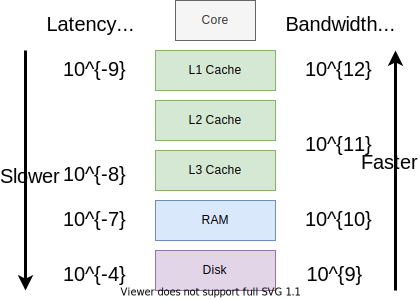
\includegraphics[width=1\textwidth]{figures/cachesketch.png}
      \end{center}
    \end{column}
  \end{columns}
  \vspace{\baselineskip}
  Optimisation: refactor algorithms to keep data in fast
  memory.

  {\footnotesize
    Check
    \href{https://colin-scott.github.io/personal_website/research/interactive_latency.html}{Colin
    Scott's page}
    for more detail on latencies.}
\end{frame}

\begin{frame}
  \frametitle{Cache memory: overview}

  \begin{exampleblock}{Features}
    \begin{itemize}[itemsep=6pt]
    \item Hierarchy of small, fast memory.
    \item Keep a copy of \emph{frequently used} data for faster access
    \end{itemize}
  \end{exampleblock}

  \pause

  \begin{challenge}{Issues}
    \begin{itemize}[itemsep=6pt]
    \item Frequently accessed data not known \emph{a priori}
    \item Only heuristics are possible $\Rightarrow$ \emph{princple of locality}
    \end{itemize}
  \end{challenge}

\end{frame}

\begin{frame}
  \frametitle{Principle of locality}
  \begin{itemize}
  \item Frequently accessed data often unknown before execution
  \item In practice, most programs exhibit \emph{locality} of data
    access.
  \item Optimised algorithms attempt to \emph{exploit} this
    locality.
  \end{itemize}

  \pause

  \begin{block}{Temporal locality}
    If I access data at some memory address, it is likely that I will
    do so again ``soon''.
  \end{block}

  \vskip -2pt

  \begin{block}{Spatial locality}
    If I access data at some memory address, it is likely that I will
    access neighbouring addresses.
  \end{block}
\end{frame}

\begin{frame}
  \frametitle{Temporal locality}

  On \structure{first access} to a new address, the data is:\\[-13pt]
  \begin{itemize}[itemsep=6pt]
  \item loaded from main memory to registers
  \item stored in cache
  \end{itemize}

  \vskip 20pt
  \pause

  \structure{Trade-off} solution:\\[-13pt]
  \begin{itemize}[itemsep=6pt]
  \item Small performance penalty for first access (storing is not free)
  \item Subsequent accesses use cached copy and are much faster.
  \end{itemize}
\end{frame}

\begin{frame}[fragile]
  \frametitle{Spatial locality}
  On \structure{first access} to a new address, the data is:\\[-13pt]
  \begin{itemize}[itemsep=6pt]
  \item loaded from main memory to registers
  \item stored in cache
  \item neighbouring addressed are also stored in cache
  \end{itemize}

  \vskip 20pt
  \pause

  \structure{Trade-off} solution:\\[-13pt]
  \begin{itemize}[itemsep=6pt]
  \item Large performance penalty for first access
  \item Subsequent accesses to neighbouring data will be fast
  \end{itemize}

\end{frame}

\begin{frame}[fragile]
  \frametitle{Example: sum reduction}
\begin{minted}{c}
                  float s[16] = 0
                  for (i = 0; i < N; i++)
                      s[i%16] += a[i];
\end{minted}

  \vskip 15pt

  \begin{itemize}[itemsep=6pt]
  \item Temporal locality
    \begin{itemize}[itemsep=4pt]
    \item 16 entries of \texttt{s} are accessed repeatedly
    \item Makes to keep all of \texttt{s} in cache
    \end{itemize}
  \item Spatial locality
    \begin{itemize}[itemsep=4pt]
    \item Contiguous entries of \texttt{a} are accessed
    \item When loading \texttt{a[i]} it makes sense to load \texttt{a[i+1]} too.
    \end{itemize}
  \end{itemize}
\end{frame}

\begin{frame}
  \frametitle{Designing a cache}
  \begin{block}{Important questions}
    \begin{enumerate}[itemsep=6pt]
    \item When we load data into the cache, where do we put it?
    \item If we have an address, how do determine if it is in the
      cache?
    \item What do we do when the cache becomes full?
    \end{enumerate}
  \end{block}

  \vskip 11pt

  \begin{itemize}[itemsep=4pt]
  \item Each datum uniquely referenced by its $K$-bit \emph{address}
  \item Need to turn this large memory address into a cache location
  \item $K$ is typically large ($\mathsf{2^{32}/2^{64}}$ addresses)
  \end{itemize}
\end{frame}

\begin{frame}
  \frametitle{Direct mapped cache}
  \begin{itemize}
  \item Cache can store $\mathsf 2^N$ bytes.
  \item Divided into \emph{blocks} (or \emph{cache lines}) each of $\mathsf 2^M$ bytes.
  \item Each address references one byte.
  \item Use $N$ bits of the address to select which slot
    in the cache to use.
  \end{itemize}

  \vskip 11pt

  \structure{Simple solution:}
\end{frame}

\begin{frame}[fragile]
  \frametitle{Direct mapped caches: indexing}
  \begin{center}
    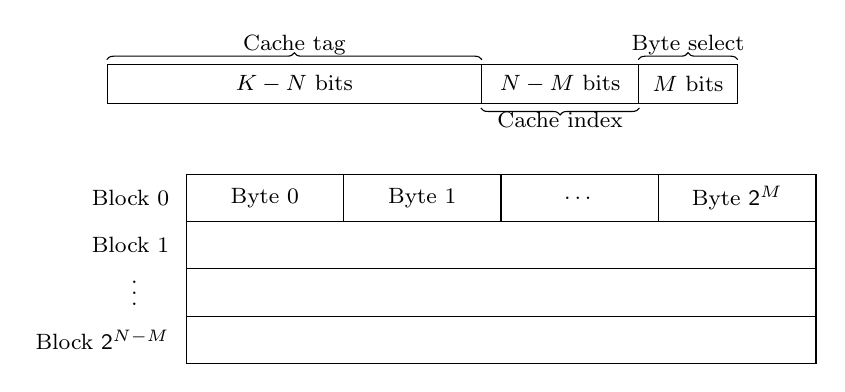
\begin{tikzpicture}
      \footnotesize \node[fit={(-1,1.5) (3.75, 2)}, inner sep=0pt,draw] (tag)
      {}; \node at (tag.center) {$K - N$ bits};
      \draw[decoration={brace,raise=0.05cm},decorate] (tag.north west) --
      (tag.north east) node [pos=0.5, anchor=south] {Cache tag};

      \node[fit={(3.75,1.5) (5.75, 2)}, inner sep=0pt,draw] (index) {}; \node at
      (index.center) {$N-M$ bits};
      \draw[decoration={brace,raise=0.05cm},decorate] (index.south east) --
      (index.south west) node[pos=0.5, anchor=north] {Cache index};

      \node[fit={(5.75,1.5) (7, 2)}, inner sep=0pt,draw] (select) {}; \node at
      (select.center) {$M$ bits}; \draw[decoration={brace,
        raise=0.05cm},decorate] (select.north west) -- (select.north east) node
      [pos=0.5, anchor=south] {Byte select};


      \node[fit={(0,0) (2,0.6)}, inner sep=0pt,draw] (byte0) {}; \node at
      (byte0.center) {Byte 0}; \node[fit={(2,0) (4,0.6)}, inner sep=0pt,draw]
      (byte1) {}; \node at (byte1.center) {Byte 1}; \node[fit={(4,0) (6,0.6)},
      inner sep=0pt,draw] (byte2) {}; \node at (byte2.center) {\dots};
      \node[fit={(6,0) (8,0.6)}, inner sep=0pt,draw] (byteM) {}; \node at
      (byteM.center) {Byte $\mathsf 2^M$};

      \node[left=0.1cm of byte0] {Block 0}; \node[fit={(0, 0) (8, -0.6)}, inner
      sep=0pt,draw] (block1) {}; \node[left=0.1cm of block1] {Block 1};
      \node[fit={(0, -0.6) (8, -1.2)}, inner sep=0pt,draw] (block2) {};
      \node[left=0.5cm of block2,yshift=0.1cm] {\vdots}; \node[fit={(0, -1.2)
        (8, -1.8)}, inner sep=0pt,draw] (blockN) {}; \node[left=0.1cm of blockN]
      {Block $\mathsf 2^{N-M}$};
    \end{tikzpicture}
  \end{center}
  \begin{itemize}
  \item \structure{Byte select}: Use lowest $M$ bits to select correct byte in block.
  \item \structure{Cache index}: Use next $N-M$ bits to select correct block.
  \item \structure{Cache tag}: Use remaining $K - N$ bits as a key.
  \end{itemize}
\end{frame}

\begin{frame}
  \frametitle{Choice of cache line size}
  \begin{itemize}[itemsep=8pt]
  \item Data is loaded one \emph{cache line} at a time
  \item Immediately exploits \emph{spatial locality}
  \item Larger cache lines are not always better
  \item Almost all modern CPUs use 64-byte size
  \end{itemize}

  \vskip 16pt

  \begin{block}{Rule of thumb}
    Cache-friendly algorithms work on cache line-sized chunks of data.
  \end{block}
\end{frame}

\begin{frame}[fragile]
  \frametitle{Direct mapped caches: eviction}
  \begin{itemize}[itemsep=4pt]
  \item \structure{Conflict:} two addresses have the same low bit pattern
  \item \structure{Resolution:} newest loaded address wins.
  \item This is a \emph{least recently used} (LRU) eviction policy.
  \end{itemize}

  \pause

  \begin{block}{What can go wrong?}
    \begin{columns}
      \begin{column}{0.45\textwidth}
\begin{minted}[fontsize=\small]{c}
int a[64], b[64], r = 0;
for (int i = 0; i < 100; i++)
   for (int j = 0; j < 64; j++)
       r += a[j] + b[j];
\end{minted}
      \end{column}
      \begin{column}{0.45\textwidth}
        \begin{itemize}
        \item 1KB cache
        \item 32-byte block size
        \item So $\mathsf{N=10, M=5}$
        \item 32 blocks in the cache
        \end{itemize}
      \end{column}
    \end{columns}
  \end{block}
\end{frame}

\newcommand{\myphantom}{\phantom{$a_{\mathsf{11:11}}$}}
\newcommand{\myvphantom}{\vphantom{$b_{\mathsf{11:11}}$}}
\newcommand{\myhphantom}{\vphantom{$a_{\mathsf{11:11}}$}}

\begin{frame}[fragile]
  \frametitle{Conflicts reduce \emph{effective} cache size}
  \begin{columns}
    \begin{column}{0.33\linewidth}
\centering
\begin{minted}[fontsize=\footnotesize]{c}
for (int j = 0; j < 64; j++)
    r += a[j] + b[j];
\end{minted}

\vskip 7pt
\small
      \begin{onlyenv}<1>
        
\begin{tikzpicture} [nodes in empty cells, nodes={minimum
            width=1.4cm, minimum height=0.7cm, inner sep=0}, row sep=-\pgflinewidth,
          column sep=-\pgflinewidth]
          border/.style={draw} \matrix(matrix)[matrix of nodes,
          nodes={draw}] {
            \myphantom&\myphantom&\myphantom&\myphantom\\
            \myphantom&\myphantom&\myphantom&\myphantom\\
            \myphantom&\myphantom&\myphantom&\myphantom\\
            \myphantom&\myphantom&\myphantom&\myphantom\\
            \myphantom&\myphantom&\myphantom&\myphantom\\
            \myphantom&\myphantom&\myphantom&\myphantom\\
            \myphantom&\myphantom&\myphantom&\myphantom\\
            \myphantom&\myphantom&\myphantom&\myphantom\\
          };
        \end{tikzpicture}
      \end{onlyenv}%
      \begin{onlyenv}<2>
        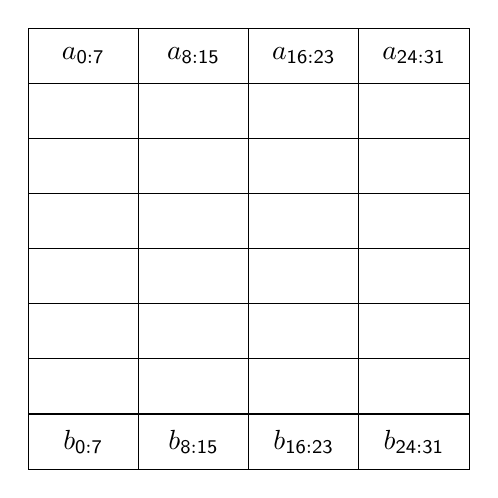
\begin{tikzpicture} [nodes in empty cells, nodes={minimum
            width=1.4cm, minimum height=0.7cm, inner sep=0}, row
          sep=-\pgflinewidth, column sep=-\pgflinewidth]
          border/.style={draw} \matrix(matrix)[matrix of nodes,
          nodes={draw}] {
            \myvphantom{}$a_{\mathsf{0:7}}$ & \myvphantom{}$a_{\mathsf{8:15}}$ &\myvphantom{}$a_{\mathsf{16:23}}$ & \myvphantom{}$a_{\mathsf{24:31}}$ \\
            \myphantom&\myphantom&\myphantom&\myphantom\\
            \myphantom&\myphantom&\myphantom&\myphantom\\
            \myphantom&\myphantom&\myphantom&\myphantom\\
            \myphantom&\myphantom&\myphantom&\myphantom\\
            \myphantom&\myphantom&\myphantom&\myphantom\\
            \myphantom&\myphantom&\myphantom&\myphantom\\
            $b_{\mathsf{0:7}}$ & $b_{\mathsf{8:15}}$ & $b_{\mathsf{16:23}}$ & $b_{\mathsf{24:31}}$ \\
          };
        \end{tikzpicture}
      \end{onlyenv}%
      \begin{onlyenv}<3>
        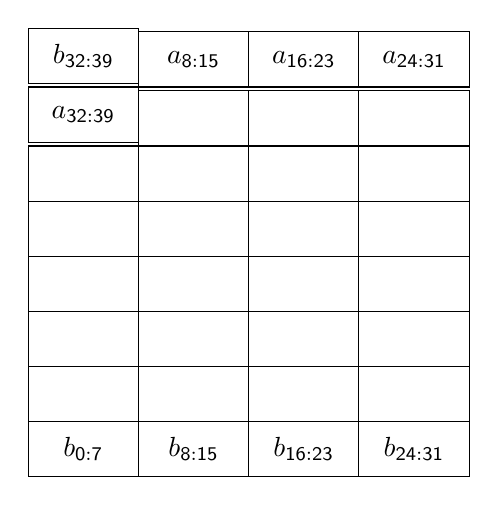
\begin{tikzpicture} [nodes in empty cells, nodes={minimum
            width=1.4cm, minimum height=0.7cm, inner sep=0}, row
          sep=-\pgflinewidth, column sep=-\pgflinewidth]
          border/.style={draw} \matrix(matrix)[matrix of nodes,
          nodes={draw}] {
            $b_{\mathsf{32:39}}$ & \myvphantom{}$a_{\mathsf{8:15}}$ & \myvphantom{}$a_{\mathsf{16:23}}$ & \myvphantom{}$a_{\mathsf{24:31}}$ \\
            $a_{\mathsf{32:39}}$&\myhphantom&\myhphantom&\myhphantom\\
            \myphantom&\myphantom&\myphantom&\myphantom\\
            \myphantom&\myphantom&\myphantom&\myphantom\\
            \myphantom&\myphantom&\myphantom&\myphantom\\
            \myphantom&\myphantom&\myphantom&\myphantom\\
            \myphantom&\myphantom&\myphantom&\myphantom\\
            $b_{\mathsf{0:7}}$   & $b_{\mathsf{8:15}}$ & $b_{\mathsf{16:23}}$ & $b_{\mathsf{24:31}}$ \\
          };
        \end{tikzpicture}
      \end{onlyenv}%
      \begin{onlyenv}<4>
        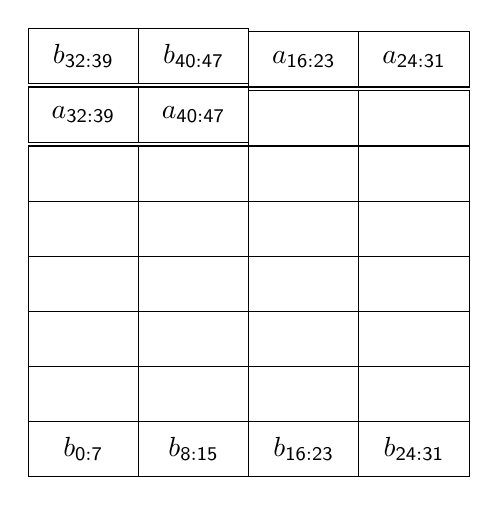
\begin{tikzpicture} [nodes in empty cells, nodes={minimum
            width=1.4cm, minimum height=0.7cm, inner sep=0}, row
          sep=-\pgflinewidth, column sep=-\pgflinewidth]
          border/.style={draw} \matrix(matrix)[matrix of nodes,
          nodes={draw}] {
            $b_{\mathsf{32:39}}$ & $b_{\mathsf{40:47}}$  & \myvphantom{}$a_{\mathsf{16:23}}$ & \myvphantom{}$a_{\mathsf{24:31}}$ \\
            $a_{\mathsf{32:39}}$ & $a_{\mathsf{40:47}}$ &\myhphantom&\myhphantom\\
            \myphantom&\myphantom&\myphantom&\myphantom\\
            \myphantom&\myphantom&\myphantom&\myphantom\\
            \myphantom&\myphantom&\myphantom&\myphantom\\
            \myphantom&\myphantom&\myphantom&\myphantom\\
            \myphantom&\myphantom&\myphantom&\myphantom\\
            $b_{\mathsf{0:7}}$   & $b_{\mathsf{8:15}}$  & $b_{\mathsf{16:23}}$ & $b_{\mathsf{24:31}}$ \\
          };
        \end{tikzpicture}
      \end{onlyenv}%
      \begin{onlyenv}<5>
        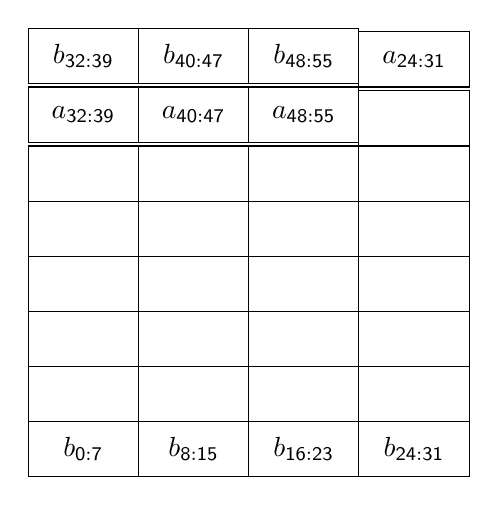
\begin{tikzpicture} [nodes in empty cells, nodes={minimum
            width=1.4cm, minimum height=0.7cm, inner sep=0}, row
          sep=-\pgflinewidth, column sep=-\pgflinewidth]
          border/.style={draw} \matrix(matrix)[matrix of nodes,
          nodes={draw}] {
            $b_{\mathsf{32:39}}$ & $b_{\mathsf{40:47}}$ & $b_{\mathsf{48:55}}$ & \myvphantom{}$a_{\mathsf{24:31}}$ \\
            $a_{\mathsf{32:39}}$ & $a_{\mathsf{40:47}}$ & $a_{\mathsf{48:55}}$ &
            \myhphantom{}\\
                        &             &             &             \\
                        &             &             &             \\
                        &             &             &             \\
                        &             &             &             \\
                        &             &             &             \\
            $b_{\mathsf{0:7}}$   & $b_{\mathsf{8:15}}$  & $b_{\mathsf{16:23}}$ & $b_{\mathsf{24:31}}$ \\
          };
        \end{tikzpicture}
      \end{onlyenv}%
      \begin{onlyenv}<6->
        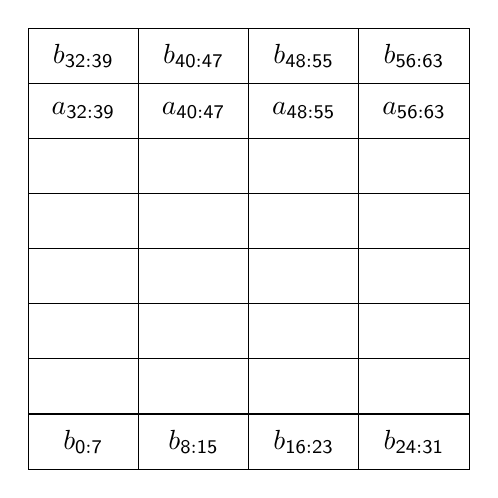
\begin{tikzpicture} [nodes in empty cells, nodes={minimum
            width=1.4cm, minimum height=0.7cm, inner sep=0}, row
          sep=-\pgflinewidth, column sep=-\pgflinewidth]
          border/.style={draw} \matrix(matrix)[matrix of nodes,
          nodes={draw}] {
            $b_{\mathsf{32:39}}$ & $b_{\mathsf{40:47}}$ & $b_{\mathsf{48:55}}$ & $b_{\mathsf{56:63}}$ \\
            $a_{\mathsf{32:39}}$ & $a_{\mathsf{40:47}}$ & $a_{\mathsf{48:55}}$ & $a_{\mathsf{56:63}}$ \\
                        &             &             &             \\
                        &             &             &             \\
                        &             &             &             \\
                        &             &             &             \\
                        &             &             &             \\
            $b_{\mathsf{0:7}}$   & $b_{\mathsf{8:15}}$  & $b_{\mathsf{16:23}}$ & $b_{\mathsf{24:31}}$ \\
          };
        \end{tikzpicture}
      \end{onlyenv}%
    \end{column}
    \begin{column}{0.45\linewidth}
\begin{minted}[fontsize=\scriptsize]{c}
&a[00] = ... 00000 00000 => block  0, byte offset 0
&a[01] = ... 00000 00100 => block  0, byte offset 4
&a[02] = ... 00000 01000 => block  0, byte offset 8
&a[03] = ... 00000 01100 => block  0, byte offset 12
&a[04] = ... 00000 10000 => block  0, byte offset 16
&a[05] = ... 00000 10100 => block  0, byte offset 20
&a[06] = ... 00000 11000 => block  0, byte offset 24
&a[07] = ... 00000 11100 => block  0, byte offset 28
...
&b[00] = ... 11100 00000 => block 28, byte offset 0
&b[01] = ... 11100 00100 => block 28, byte offset 4
&b[02] = ... 11100 01000 => block 28, byte offset 8
&b[03] = ... 11100 01100 => block 28, byte offset 12
&b[04] = ... 11100 10000 => block 28, byte offset 16
&b[05] = ... 11100 10100 => block 28, byte offset 20
&b[06] = ... 11100 11000 => block 28, byte offset 24
&b[07] = ... 11100 11100 => block 28, byte offset 28
...
\end{minted}
    \end{column}
  \end{columns}
\end{frame}
\begin{frame}[fragile]
  \frametitle{Cache thrashing}
  \begin{block}{What can go wrong?}
    \begin{columns}
      \begin{column}{0.45\textwidth}
\begin{minted}[fontsize=\scriptsize]{c}
int A[64], B[64], r = 0;
for (int i = 0; i < 100; i++)
   for (int j = 0; j < 64; j++)
       r += A[j] + B[j];
\end{minted}
      \end{column}
      \begin{column}{0.45\textwidth}
        \begin{itemize}
        \item 1KB cache
        \item 32 byte block size
        \item So $N=10$, $M=5$. \\32 blocks in the cache.
        \end{itemize}
      \end{column}
    \end{columns}
  \end{block}


    \begin{itemize}
    \item We need $\mathsf{2 \cdot 64 \cdot 4 = 512}$ bytes to store $A$ and $B$
      in cache.
\item This only requires 16 blocks, so our cache is large enough.
    \item If low bits of addresses match, same cache lines are mapped.
    \item In the worst case, every load of \texttt{B[j]} evicts
      \texttt{A[j]}, and vice versa.
    \end{itemize}

\end{frame}

\begin{frame}[t]
  \frametitle{Cache associativity}
  \begin{itemize}[itemsep=8pt]
  \item Direct mapped
    \begin{itemize}[wide=0pt,itemsep=6pt]
    \item Each RAM \emph{block} maps to exactly one cache
      line.
    \item LRU eviction policy (new data overwrite old)
    \end{itemize}
  \item<2> Fully associative
    \begin{itemize}[wide=0pt,itemsep=6pt]
    \item Each RAM \emph{byte} can map to any cache line
    \item Data is stored in first unused cache line
    \item If all lines are used, overall LRU one is replaced
    \item Most flexible, but also mostexpensive
    \end{itemize}
  \end{itemize}
\end{frame}

\begin{frame}
  \frametitle{$k$-way set associative cache}
    \begin{itemize}[itemsep=8pt]
    \item $k$ ``copies'' of a direct mapped cache.  Each block from main
      memory maps to one of $k$ cache lines, called \emph{sets}.
    \item Typically use LRU eviction.
    \item Usual choice: $N \in \{2, 4, 8, 16\}$.
    \item Skylake has $N = 8$ for L1, $N = 16$ for L2, $N = 11$
      for L3.
    \end{itemize}
\end{frame}

\begin{frame}
  \frametitle{Exercise: cache and memory bandwidth}
  \begin{enumerate}[itemsep=8pt]
    \item Split into small groups
    \item Make sure one person per group has access to Hamilton
    \item Benchmark memory bandwidth as a function of vector size
    \item You can use the bash script from last week.
    \item Ask questions!
    \end{enumerate}
  \end{frame}

\begin{frame}
  \frametitle{Results}
  \pgfplotsset{
    execute at begin axis={
      \pgfplotsset{
        width=.8\textwidth,
        height=.8\textheight,
      }
    }
  }
  \begin{center}
    \begin{tikzpicture}
      \begin{axis}[xlabel={Bytes},
        ylabel near ticks,
        axis y line*=left,
        ylabel={MByte/s},
        xmode=log,
        xtick={1,1024,1024*1024},
        xticklabels={1kB,1MB,1GB},
        log basis x={10},
        legend style={
          cells={
            anchor=west,
            align=left},
          fill=bgcolor},]
        \pgfplotstableread[row sep=\\]{%
          Bytes clcopy clload clstore\\
          1 139535.62 179003.98 134269.99
          2 196072.14 203681.02 169971.85\\
          4 283292.66 273443.12 190373.63\\
          8 344672.52 325878.19 201236.47\\
          16 381529.82 358668.46 206621.30\\
          32 376355.40 321852.29 189942.49\\
          64 104077.55 103779.30 103850.40\\
          128 105189.99 105002.13 105069.61\\
          256 103963.27 105435.72 105473.81\\
          512 96728.33 97349.98 101997.74\\
          1024 81027.42 79056.48 95002.92\\
          2048 79067.36 78479.83 94617.17\\
          4096 78963.31 78506.96 86539.01\\
          8192 79746.77 95353.00 84450.10\\
          16384 44177.92 59154.62 46998.52\\
          32768 17845.85 16425.60 12484.70\\
          65536 18091.12 16483.60 12538.13\\
          131072 17937.64 16484.62 12566.02\\
          262144 17954.16 16564.25 12524.69\\
          524288 17899.87 16464.03 12552.42\\
          1048576 17847.05 16443.76 12518.28\\
        }\mydata
        \addplot [Red, very thick, mark=*] table[x=Bytes,y=clcopy] {\mydata};\label{clcopy}
        \addlegendentry{\texttt{clcopy}}
        \addplot [Blue, very thick, mark=square] table[x=Bytes,y=clload] {\mydata};\label{clload}
        \addlegendentry{\texttt{clload}}
        \addplot [Green, very thick, mark=diamond] table[x=Bytes,y=clstore]
        {\mydata};\label{clstore}
        \addlegendentry{\texttt{clstore}}

        \only<2>{%
          \addlegendimage{/pgfplots/refstyle=sum-sp-avx}
          \addlegendentry{\texttt{sum\_sp\_avx}}
        }

      \end{axis}
      \pause
      \begin{axis}[xlabel={},
        ylabel near ticks,
        axis y line*=right,
        ylabel={MFlops/s},
        xmode=log,
        xticklabels={},
        log basis x={2},
        legend pos={outer north east},
        legend style={cells={anchor=west, align=left}},]
        \pgfplotstableread[row sep=\\]{%
          Bytes scalar avx\\
          1 4721.23 25633.48\\
          2 4566.17 35462.91\\
          4 4497.61 40717.13\\
          8 4465.51 37820.79\\
          16 4443.53 36595.48\\
          32 4424.07 33791.29\\
          64 4222.61 25780.94\\
          128 4258.17 26158.12\\
          256 4204.51 26281.52\\
          512 4384.87 23034.10\\
          1024 4394.45 18759.08\\
          2048 4386.30 18655.37\\
          4096 4396.57 18868.36\\
          8192 4398.89 18856.77\\
          16384 4084.19 13711.12\\
          32768 3387.52 5583.20\\
          65536 3399.47 5633.13\\
          131072 3412.19 5582.03\\
          262144 3399.07 5573.66\\
          524288 3404.33 5581.31\\
          1048576 3428.27 5645.72\\
        }\mydata

        % \addlegendimage{/pgfplots/refstyle=clcopy}
        % \addlegendentry{\texttt{clcopy}}
        % \addlegendimage{/pgfplots/refstyle=clload}
        % \addlegendentry{\texttt{clload}}
        % \addlegendimage{/pgfplots/refstyle=clstore}
        % \addlegendentry{\texttt{clstore}}

        \addplot [black, mark=x, thick] table[x=Bytes,y=avx] {\mydata}; \label{sum-sp-avx}
        % \addlegendentry{test};
      \end{axis}
    \end{tikzpicture}
  \end{center}
\end{frame}

\begin{frame}
  \frametitle{Interpretation}
  \begin{itemize}
  \item Vectorised addition requires 1 32Byte load/cycle (for the 8
    floats)
  \item Accumulation parameter held in a register.
  \item[$\Rightarrow$] requires sustained load bandwidth of $32\times
    2.9 = 92.8$GByte/s
  \item From L1 (less than 32kB) we see sustained bandwidth of around
    300GByte/s $\Rightarrow$ floating-point throughput is limit.
  \item L2 (less than 256kB) provides around 80GByte/s or around
    27Bytes/cycle $\Rightarrow$ 6.75 floats/cycle $\Rightarrow$ peak
    is around 19GFlops/s.
  \item L3 (less than 30MB) provides around 36GByte/s or around
    12Bytes/cycle $\Rightarrow$ 2.75 floats/cycle $\Rightarrow$ peak
    is around 8GFlops/s.
  \item Main memory provides around 13GByte/s or around 4.5Bytes/cycle
    $\Rightarrow$ 1.1floats/cycle $\Rightarrow$ peak is around 3.25GFlops/s.
  \end{itemize}
\end{frame}

\begin{frame}
  \frametitle{Adding bandwidth-induced limits}
  Not bad for a pen-and-paper exercise.
  \begin{center}
    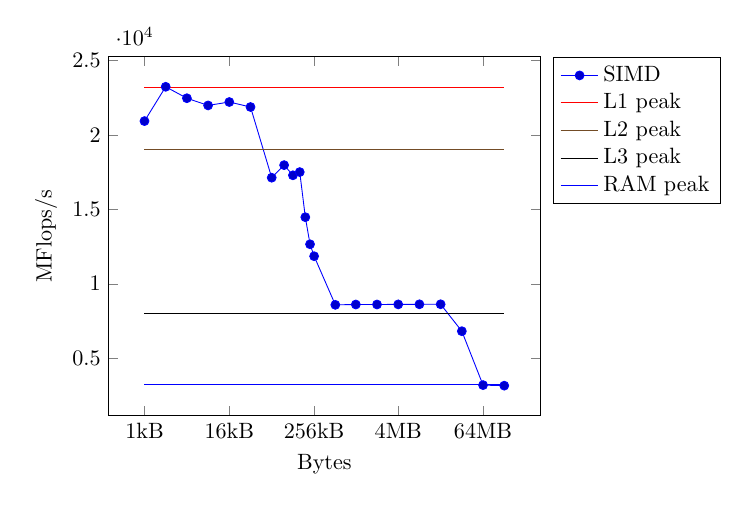
\begin{tikzpicture}[scale=0.8]
      \begin{axis}[xlabel={Bytes},
        ylabel near ticks,
        ylabel={MFlops/s},
        xmode=log,
        xtick={1e3,16e3,256e3,4e6,64e6},
        xticklabels={1kB,16kB,256kB,4MB,64MB},
        log basis x={10},
        legend pos={outer north east},
        legend style={cells={anchor=west, align=left}},]
        \pgfplotstableread[row sep=\\]{%
          Bytes MFlops Peak L2Peak L3Peak RAMPeak\\
          1e3 20934.77 23.2e3 19e3 8e3 3.25e3\\
          2e3 23240.25 23.2e3 19e3 8e3 3.25e3\\
          4e3 22471.22 23.2e3 19e3 8e3 3.25e3\\
          8e3 21988.17 23.2e3 19e3 8e3 3.25e3\\
          16e3 22216.43 23.2e3 19e3 8e3 3.25e3\\
          32e3 21881.05 23.2e3 19e3 8e3 3.25e3\\
          64e3 17130.67 23.2e3 19e3 8e3 3.25e3\\
          96e3 17975.12 23.2e3 19e3 8e3 3.25e3\\
          128e3 17291.29 23.2e3 19e3 8e3 3.25e3\\
          160e3 17507.30 23.2e3 19e3 8e3 3.25e3\\
          192e3 14476.12 23.2e3 19e3 8e3 3.25e3\\
          224e3 12656.81 23.2e3 19e3 8e3 3.25e3\\
          256e3 11854.84 23.2e3 19e3 8e3 3.25e3\\
          512e3 8585.19 23.2e3 19e3 8e3 3.25e3\\
          1e6 8607.97 23.2e3 19e3 8e3 3.25e3\\
          2e6 8609.45 23.2e3 19e3 8e3 3.25e3\\
          4e6 8615.55 23.2e3 19e3 8e3 3.25e3\\
          8e6 8622.28 23.2e3 19e3 8e3 3.25e3\\
          16e6 8624.76 23.2e3 19e3 8e3 3.25e3\\
          32e6 6814.45 23.2e3 19e3 8e3 3.25e3\\
          64e6 3190.88 23.2e3 19e3 8e3 3.25e3\\
          128e6 3153.69 23.2e3 19e3 8e3 3.25e3\\}\avxdata
        \addplot+ table[x=Bytes,y=MFlops] {\avxdata};
        \addlegendentry{SIMD}
        \addplot+[mark=none] table[x=Bytes, y={Peak}] {\avxdata};
        \addlegendentry {L1 peak}
        \addplot+[mark=none] table[x=Bytes, y={L2Peak}] {\avxdata};
        \addlegendentry {L2 peak}
        \addplot+[mark=none] table[x=Bytes, y={L3Peak}] {\avxdata};
        \addlegendentry {L3 peak}
        \addplot+[mark=none] table[x=Bytes, y={RAMPeak}] {\avxdata};
        \addlegendentry {RAM peak}
      \end{axis}
    \end{tikzpicture}
  \end{center}
\end{frame}
\begin{frame}
  \frametitle{Memory/node topology}
  \texttt{likwid-topology} reports an ASCII version of diagrams like
  this.
  \begin{center}
    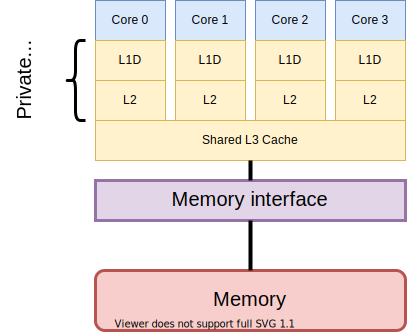
\includegraphics[height=0.5\textheight]{figures/cacheschematic.png}
  \end{center}
\end{frame}

\begin{frame}
  \frametitle{More than one core}
  \begin{itemize}
  \item So far, just looked at performance when we use a single core.
  \item In practice, most scientific computing algorithms will be
    parallel
  \item[$\Rightarrow$] How does this affect the performance?
  \end{itemize}

  \begin{answer}{Scalable vs.~Saturating}
    CPU cores are a \emph{scalable} resource.

    Adding a second core doubles the number of floating point
    operations we can perform.

    Memory bandwidth is a \emph{saturating resource}. Outside of L2
    cache (L3, main memory), CPU cores compete for the same resource.
  \end{answer}
\end{frame}

\begin{frame}
  \frametitle{Scalable vs.~Saturating}
  \begin{columns}
    \begin{column}{0.45\textwidth}
      Shared resources might show saturating performance
      \begin{tikzpicture}
        \pgfplotstableread[row sep=\\]{%
          Cores Perf\\
          1 3\\
          2 6\\
          3 8\\
          4 9\\
          5 9.4\\
          6 9.5\\
          7 9.55\\
          8 9.56\\}\saturating
        \begin{axis}[xlabel=Cores,
          ylabel=Performance,
          width=\textwidth,height=0.7\textheight]
          \addplot+ table[x=Cores, y=Perf] {\saturating};
        \end{axis}
      \end{tikzpicture}
    \end{column}
    \begin{column}{0.45\textwidth}
      Parallel resources show scalable performance
      \begin{tikzpicture}
        \pgfplotstableread[row sep=\\]{%
          Cores Perf\\
          1 1.5\\
          2 3\\
          3 4.5\\
          4 6\\
          5 7.5\\
          6 9\\
          7 10.5\\
          8 12\\}\scaling
        \begin{axis}[xlabel=Cores,
          ylabel=Performance,
          width=\textwidth,height=0.7\textheight]
          \addplot+ table[x=Cores, y=Perf] {\scaling};
        \end{axis}
      \end{tikzpicture}
    \end{column}
  \end{columns}
\end{frame}

\begin{frame}
  \frametitle{Exercise: memory bandwidth saturation}
  \begin{itemize}
  \item Goal is to benchmark the memory bandwidth for different vector
    sizes as a function of number of cores
  \item Will then look at scaling of sum reduction with cores
  \item[$\Rightarrow$] over to you.
  \end{itemize}
  \begin{center}
    Exercises at

    \url{teaching.wence.uk/comp52315/exercises/exercise03/}
  \end{center}
\end{frame}

\begin{frame}
  \frametitle{Conclusions on hardware architecture}
  \begin{challenge}{Performance considerations}
    \begin{itemize}
    \item How many instructions are required to implement an algorithm
    \item How efficiently those instructions are executed on a
      processor
    \item The runtime contribution of the data transfers
    \end{itemize}
  \end{challenge}
  \begin{answer}{Complex ``topology'' of hardware}
    \begin{itemize}
    \item Many layers of parallelism in modern hardware
    \item Sockets: around 1-4 CPUs on a typical motherboard
    \item Cores: around 4-32 cores in a typical CPU
    \item SIMD/Vectorisation: typically 2-16 single precision elements
      in vector registers on CPUs
    \item Superscalar execution: typically 2-8 instructions per cycle
    \end{itemize}
  \end{answer}
\end{frame}
\begin{frame}
  \frametitle{Challenges for program development}
  \begin{itemize}
  \item We will focus most of our efforts on SIMD and some superscalar
    execution here.
  \item An ongoing challenge is that most programming models do not
    offer a lot of explicit access to parallelism.
  \item[$\Rightarrow$] will look at mechanisms to convince compilers
    to ``do the right thing''.
  \end{itemize}
\end{frame}
\end{document}
